% !TeX root = ../main.tex
\section{Additional Real-Data Figures}
\label{app:data_plots}

\subsection{Air Quality Data: ADMM Benchmark Fits}
\label{app:spod_admm}

This appendix reports the ADMM benchmark fits of Section~\ref{sec:app:spod} and the detrended series they produce, laid out as Figures~\ref{fig:spod_quantiles_pmala} and~\ref{fig:spod_detrended_pmala}.

\begin{figure}[!ht]
	\centering
	\begin{subfigure}{0.72\textwidth}
		\centering
		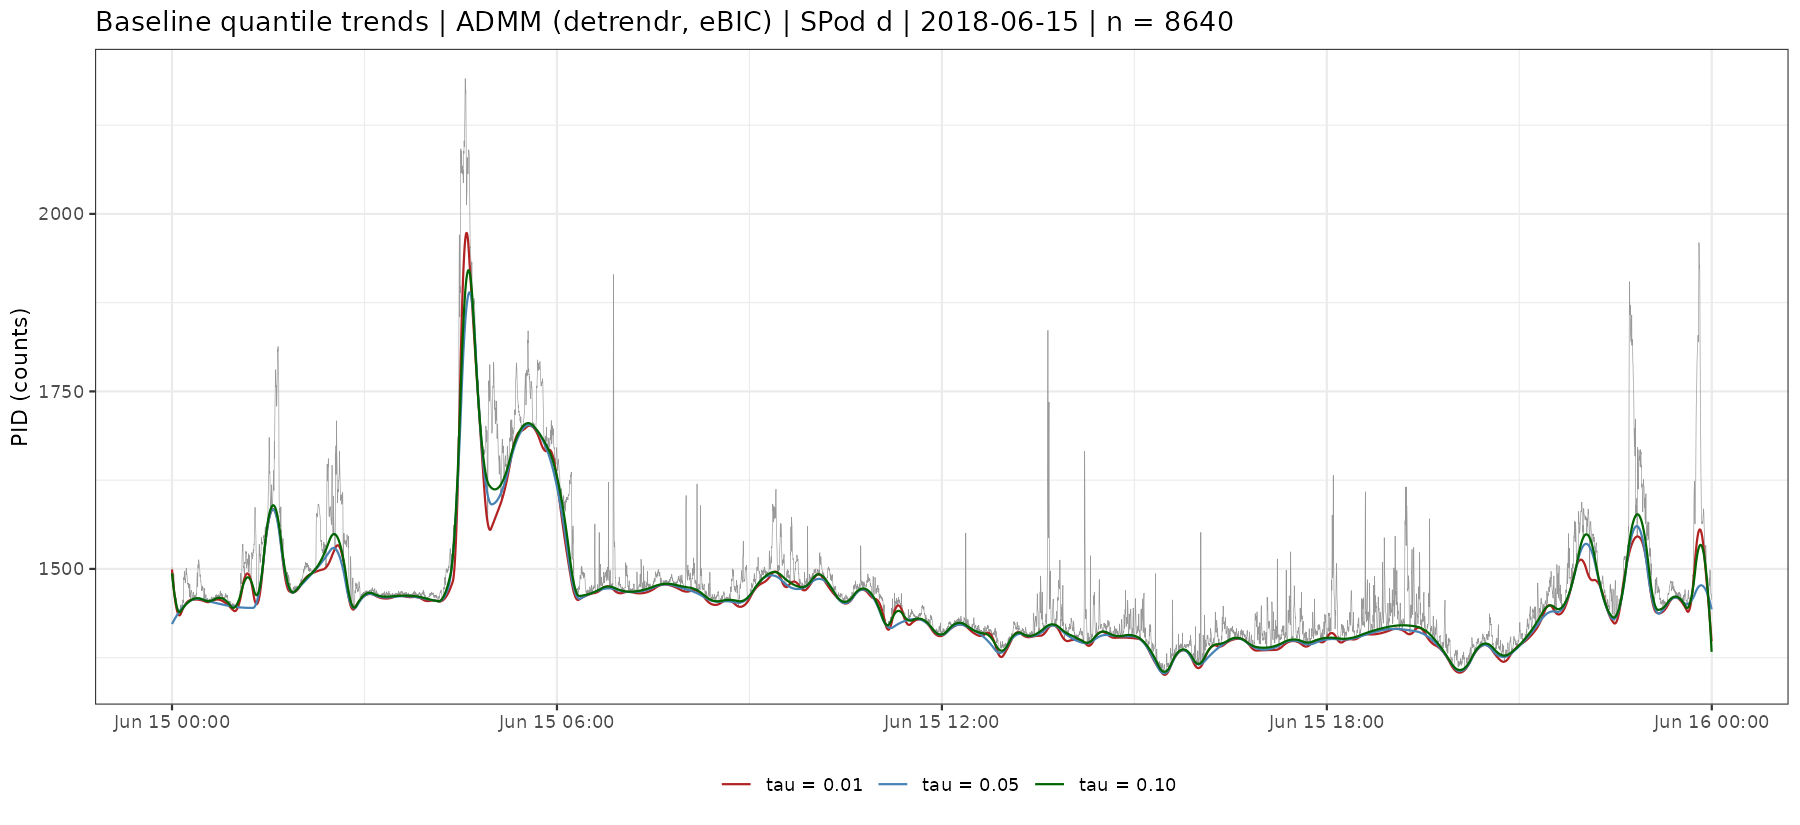
\includegraphics[width=\textwidth]{figures/spod_quantiles_admm}
		\caption{Baseline trends at $\tau \in \{0.01, 0.05, 0.1\}$, with $\lambda = 54.6$ at $\tau = 0.01$ and $\lambda = 1096.6$ at $\tau \in \{0.05, 0.1\}$ selected by eBIC.}
		\label{fig:spod_quantiles_admm}
	\end{subfigure}
	\par\medskip
	\begin{subfigure}{0.72\textwidth}
		\centering
		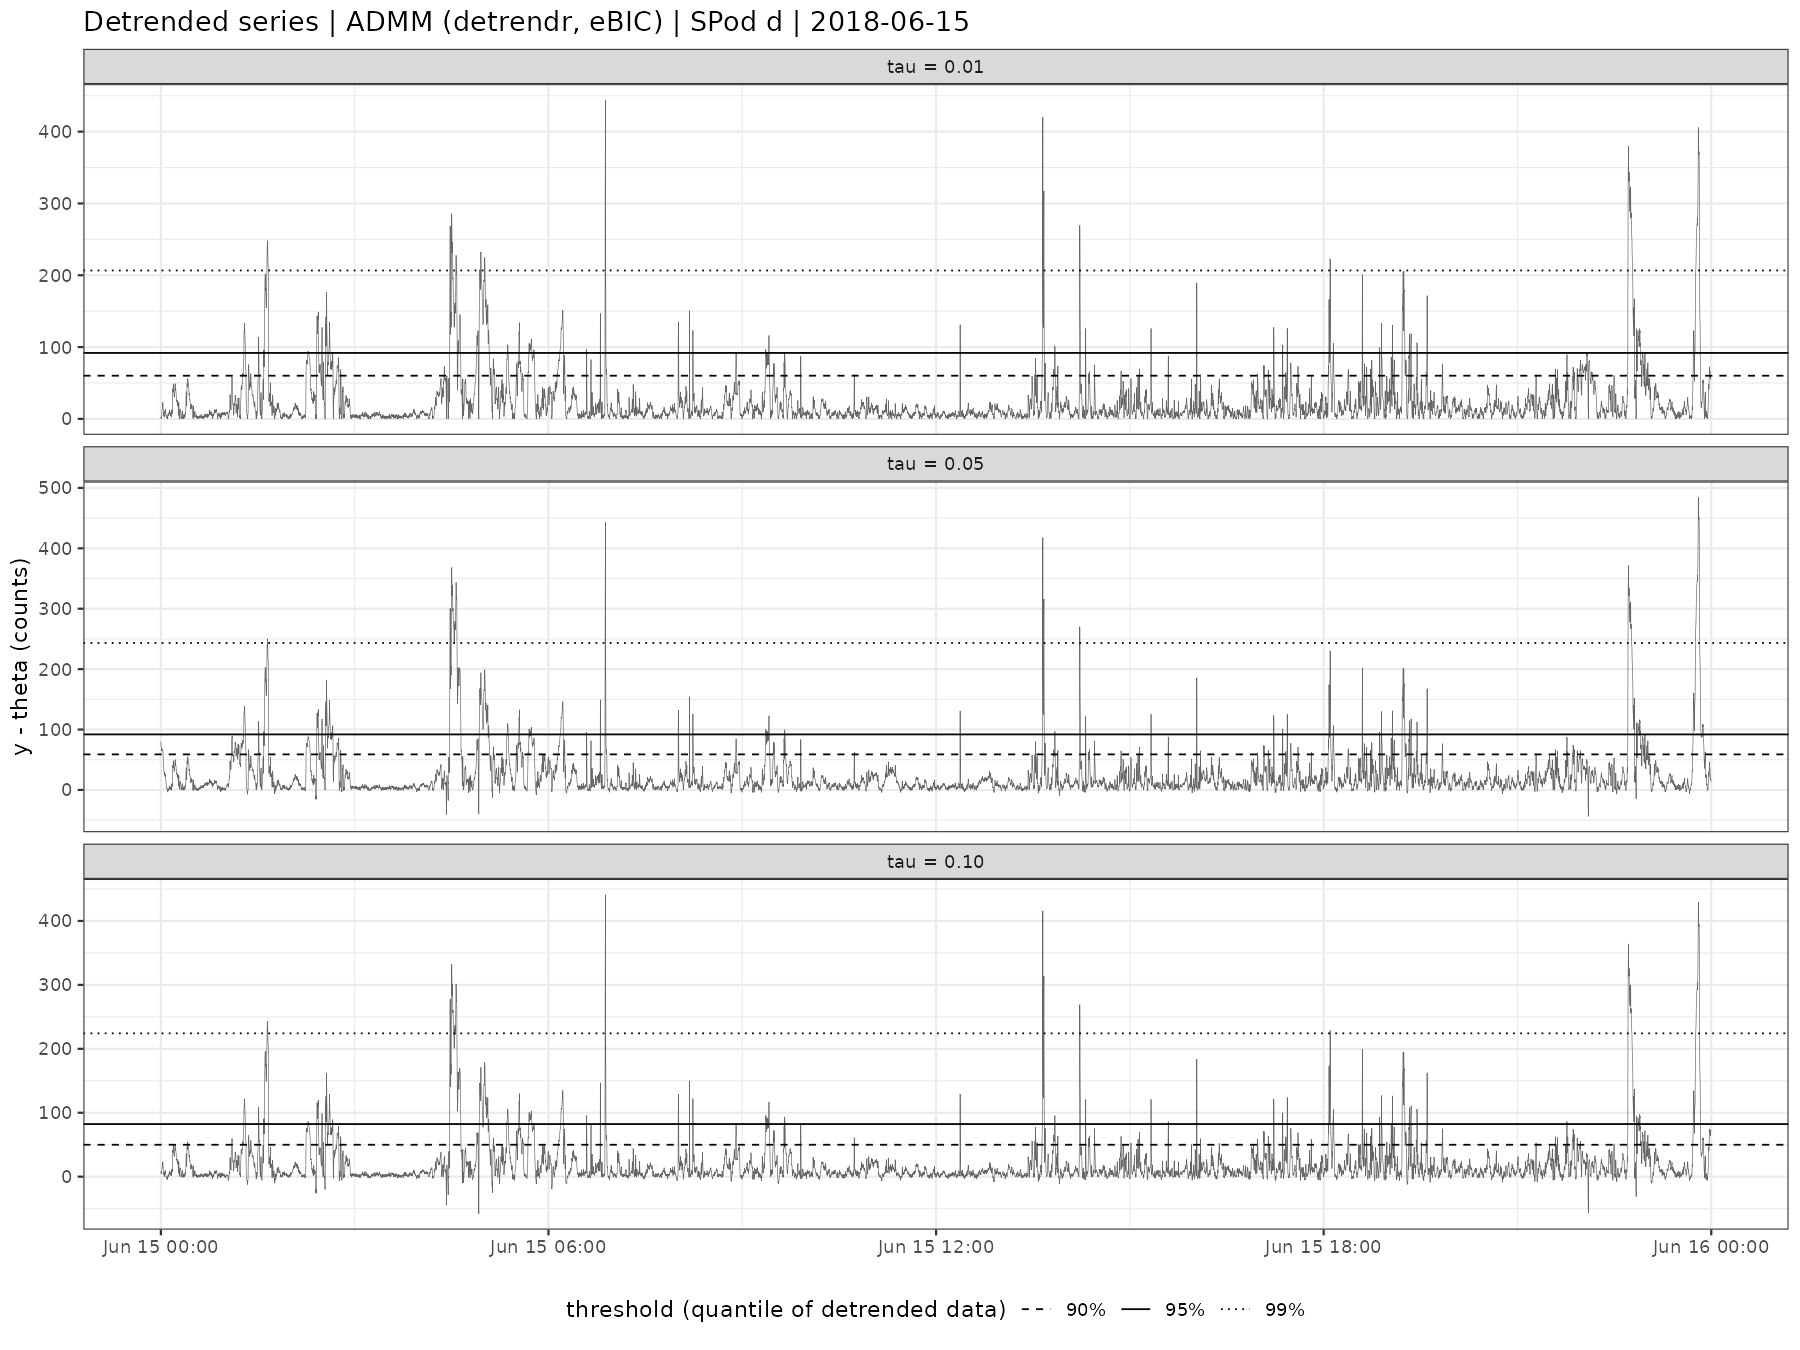
\includegraphics[width=\textwidth]{figures/spod_detrended_admm}
		\caption{Detrended series $\by - \widehat{\btheta}$ for the baselines in (a), one panel per quantile level. Horizontal lines mark the 90th (dashed), 95th (solid), and 99th (dotted) empirical percentiles of the detrended data.}
		\label{fig:spod_detrended_admm}
	\end{subfigure}
	\caption{Air quality data: ADMM benchmark fits \citep{brantley2020baseline} on the 10-second means ($n = 8{,}640$) of SPod \texttt{d}, June 15, 2018, with $\lambda$ selected by eBIC. The layout is that of Figures~\ref{fig:spod_quantiles_pmala} and~\ref{fig:spod_detrended_pmala}.}
	\label{fig:spod_admm}
\end{figure}

\clearpage

% ----------------------------------------------------------------------------
% Diagnostics from the earlier (k = 2, 60,000-iteration) Nile run.
% Parked here; the figure files are still in figures/.
% (Munich rent application removed from the paper 2026-10-28.)
% ----------------------------------------------------------------------------
\iffalse This appendix collects all plots for the real-data applications. The fits use the unchanged application P-MALA/Gibbs sampler for 60,000 iterations, with 10,000 burn-in iterations and thinning by 10.

\begin{figure}[p]
	\centering
	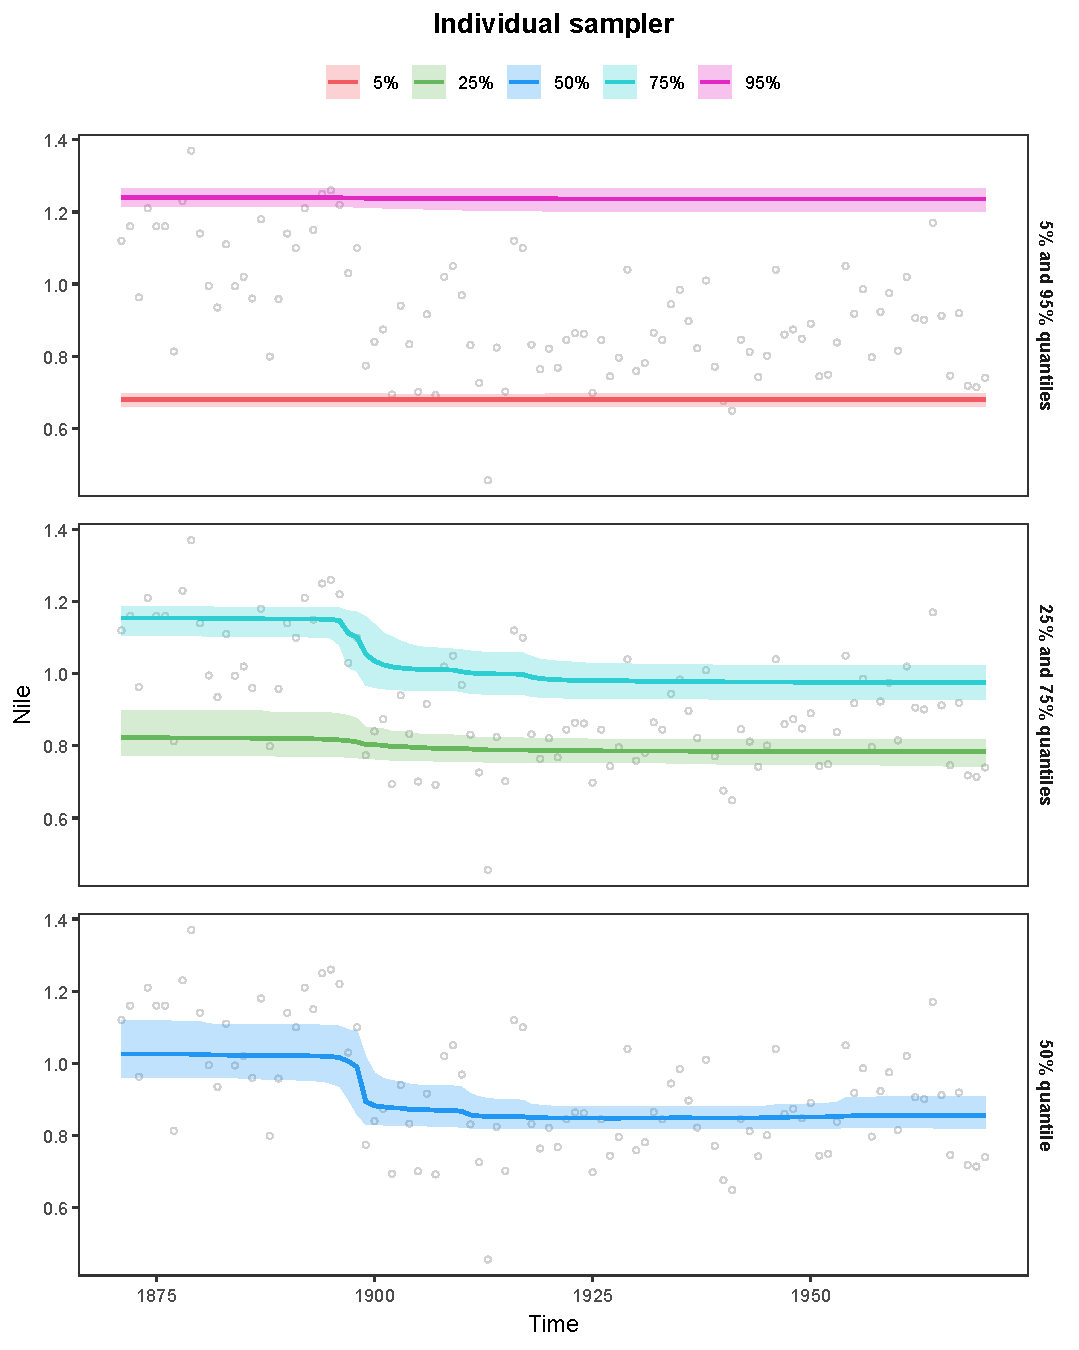
\includegraphics[width=0.75\textwidth,height=0.82\textheight,keepaspectratio]{figures/nile_individual_sampler}
	\caption{Individual P-MALA/Gibbs fits for the Nile data. Solid curves are posterior means and ribbons are 95\% pointwise credible intervals from the 5,000 retained draws. Grey circles are the rescaled observations.}
	\label{fig:nile}
\end{figure}

\begin{figure}[p]
	\centering
	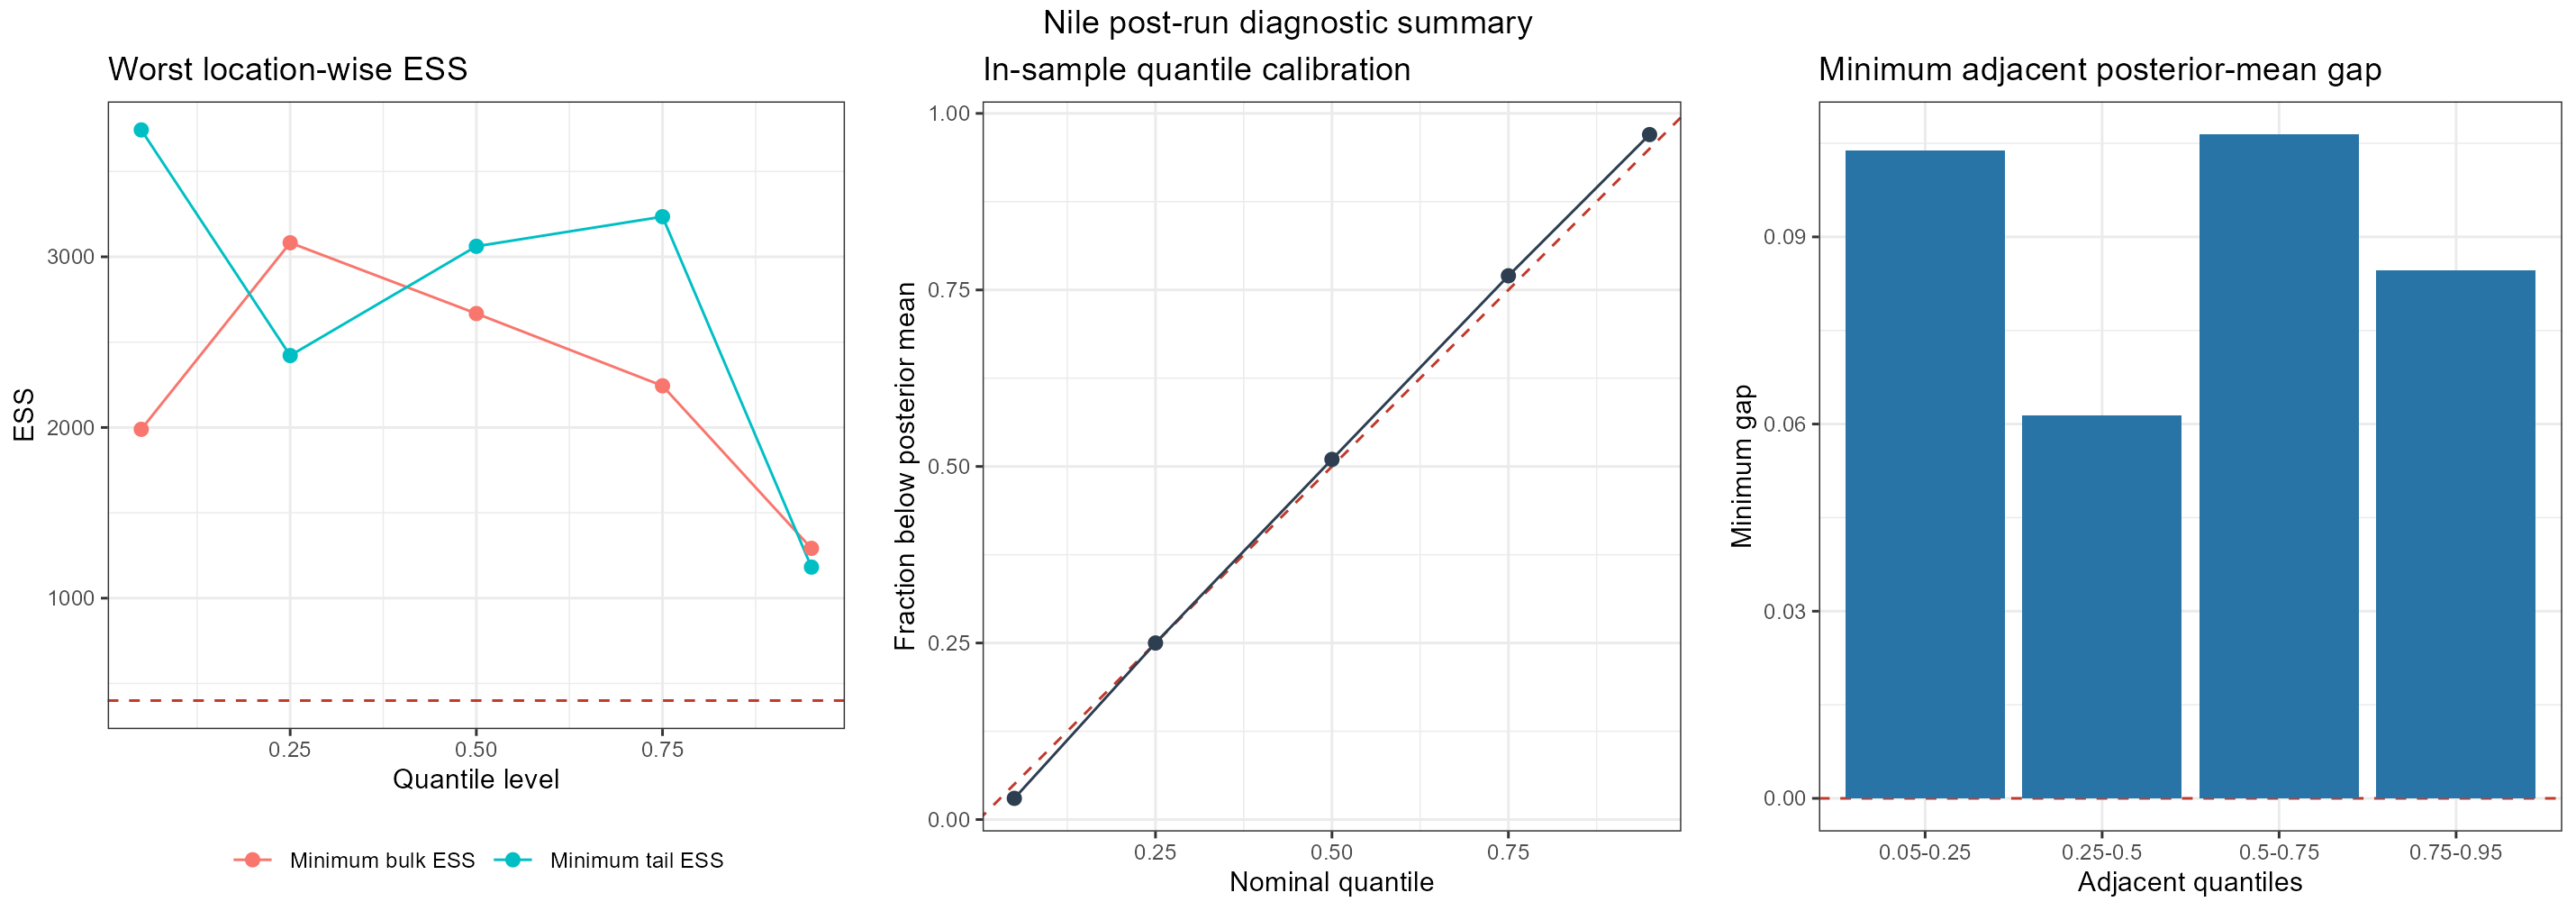
\includegraphics[width=0.75\textwidth]{figures/nile_diagnostic_summary}
	\caption{Nile post-run summaries: worst location-wise bulk and tail ESS, in-sample calibration, and minimum gap between adjacent posterior-mean curves. The ESS reference line is 400 and the calibration reference is the identity line.}
	\label{fig:app_diag_summary}
\end{figure}

\begin{figure}[p]
	\centering
	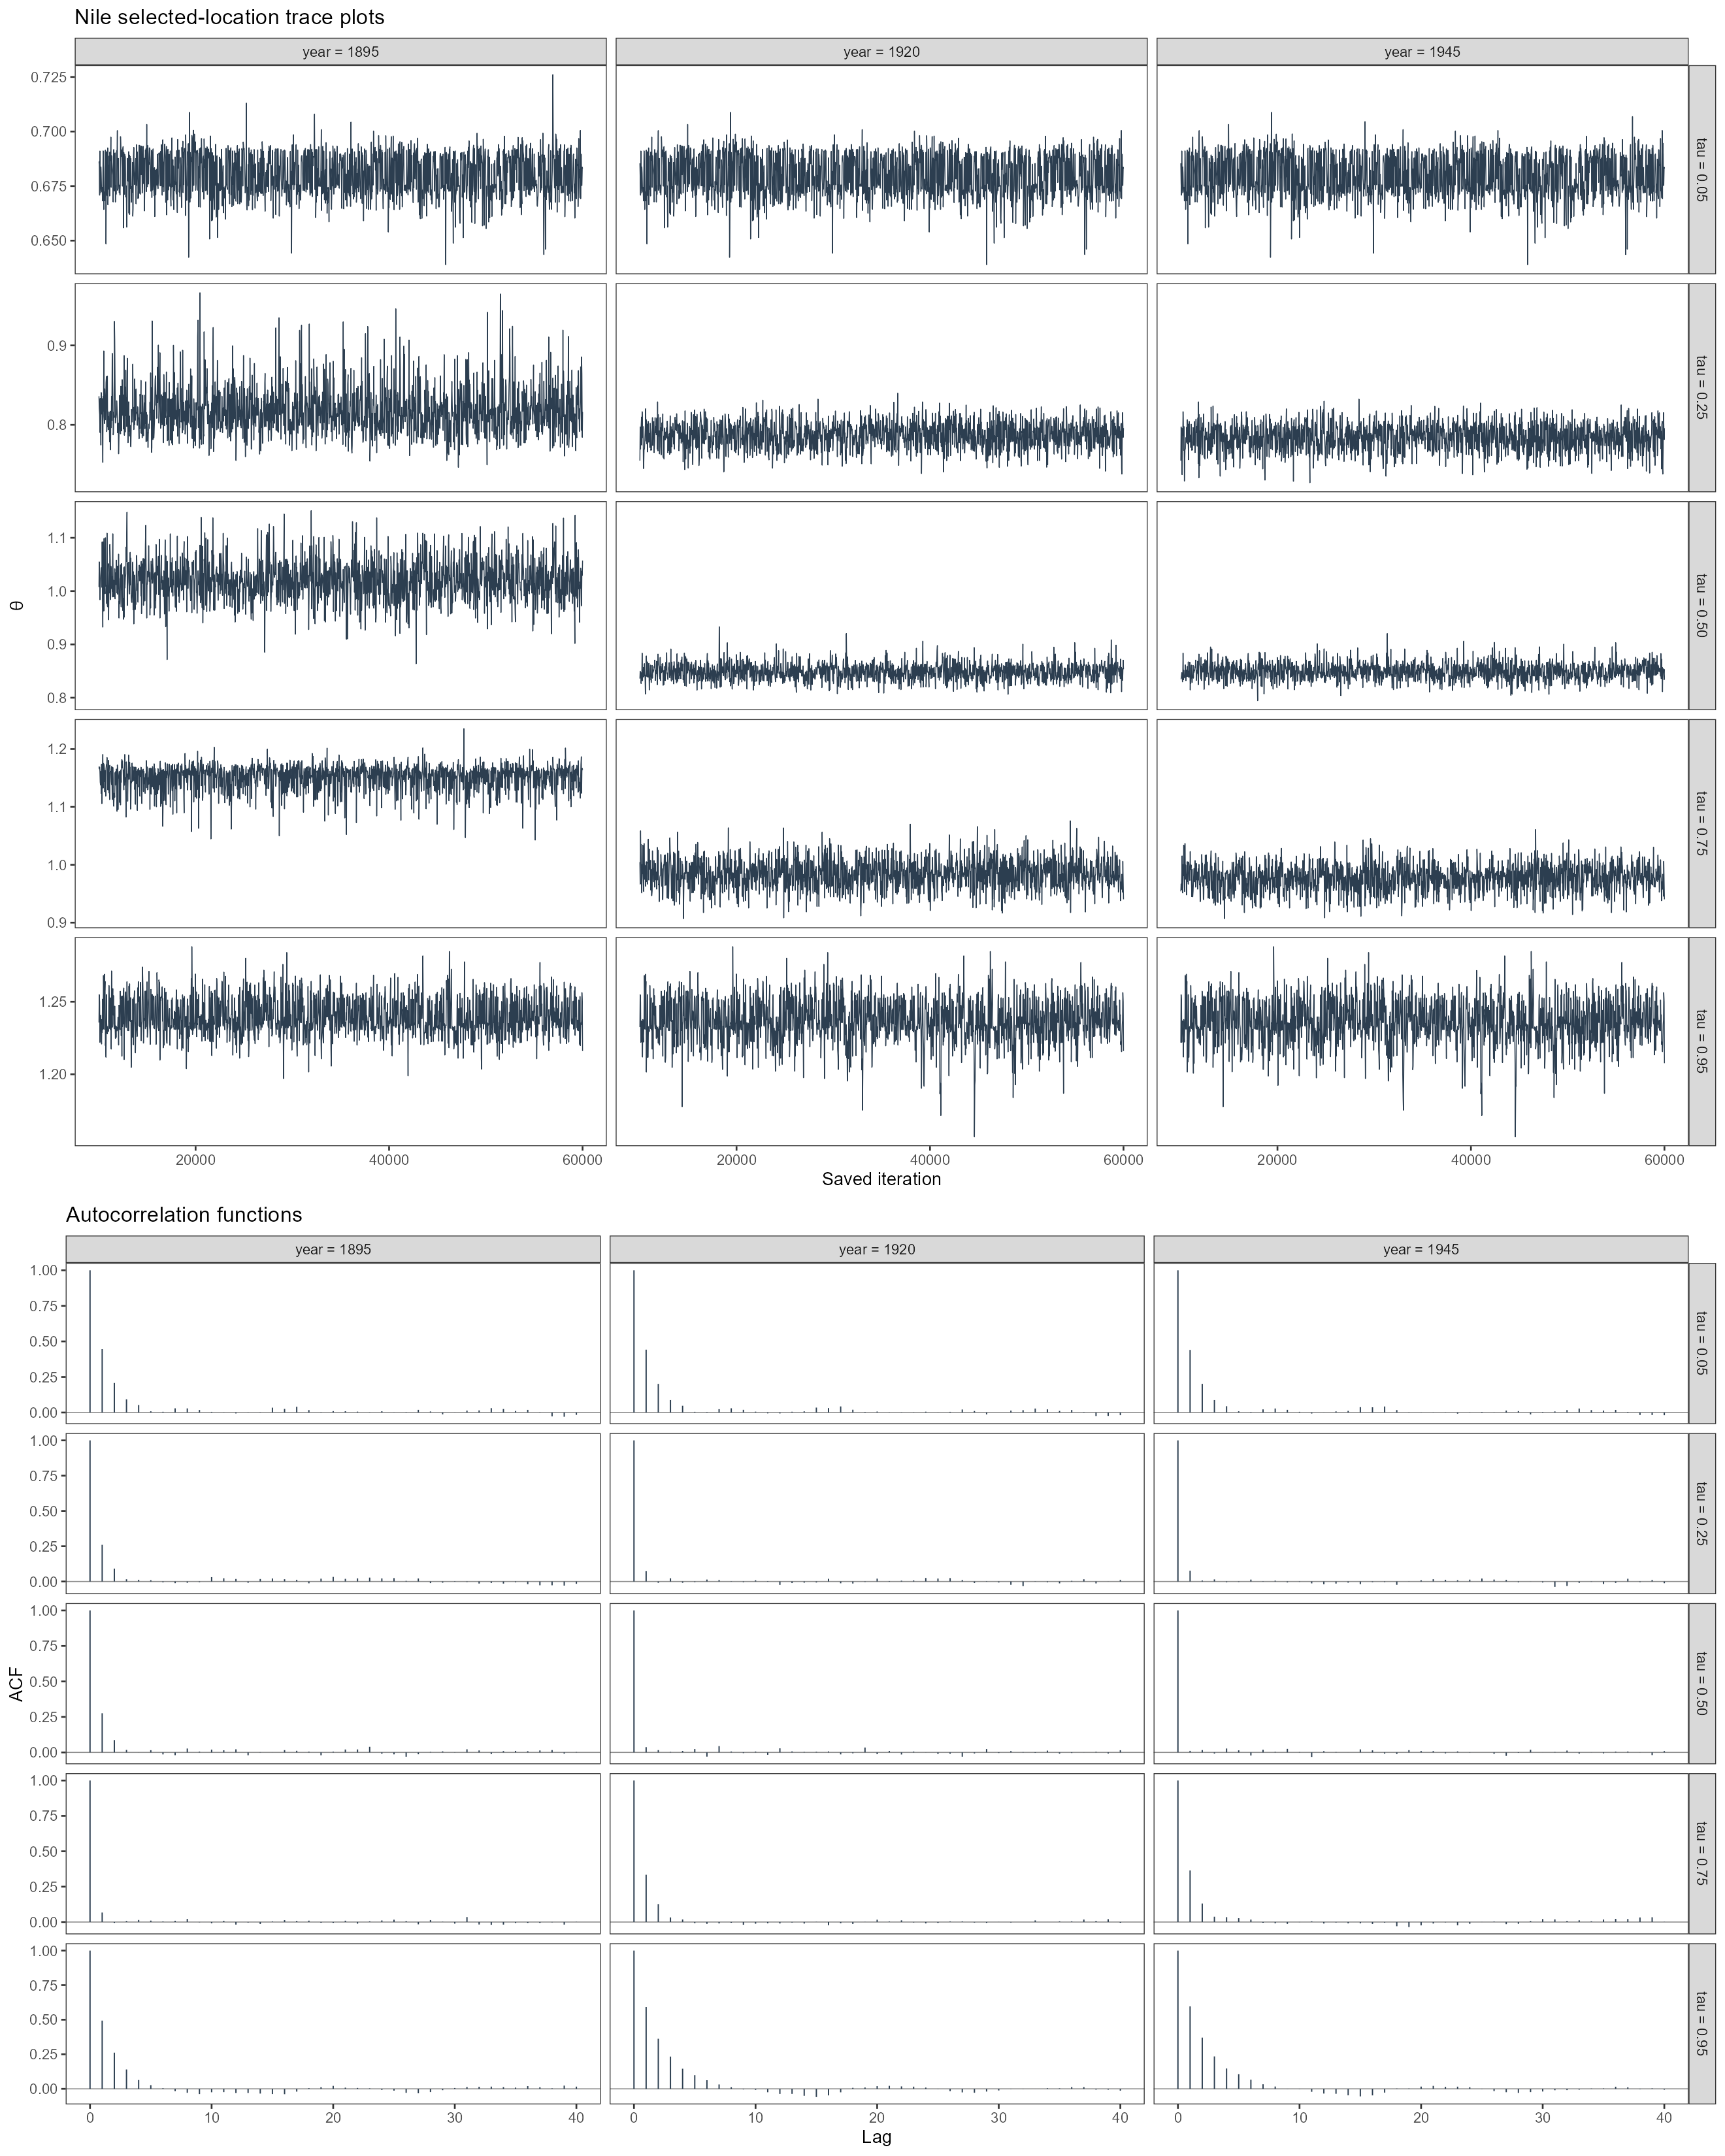
\includegraphics[width=0.75\textwidth,height=0.88\textheight,keepaspectratio]{figures/nile_trace_acf_diagnostics}
	\caption{Nile coefficient trace and autocorrelation diagnostics at representative years 1895, 1920, and 1945 for all five quantile levels. The horizontal scale of the trace panels is the original Gibbs iteration, so adjacent plotted values are ten iterations apart.}
	\label{fig:nile_trace_acf}
\end{figure}

\begin{figure}[p]
	\centering
	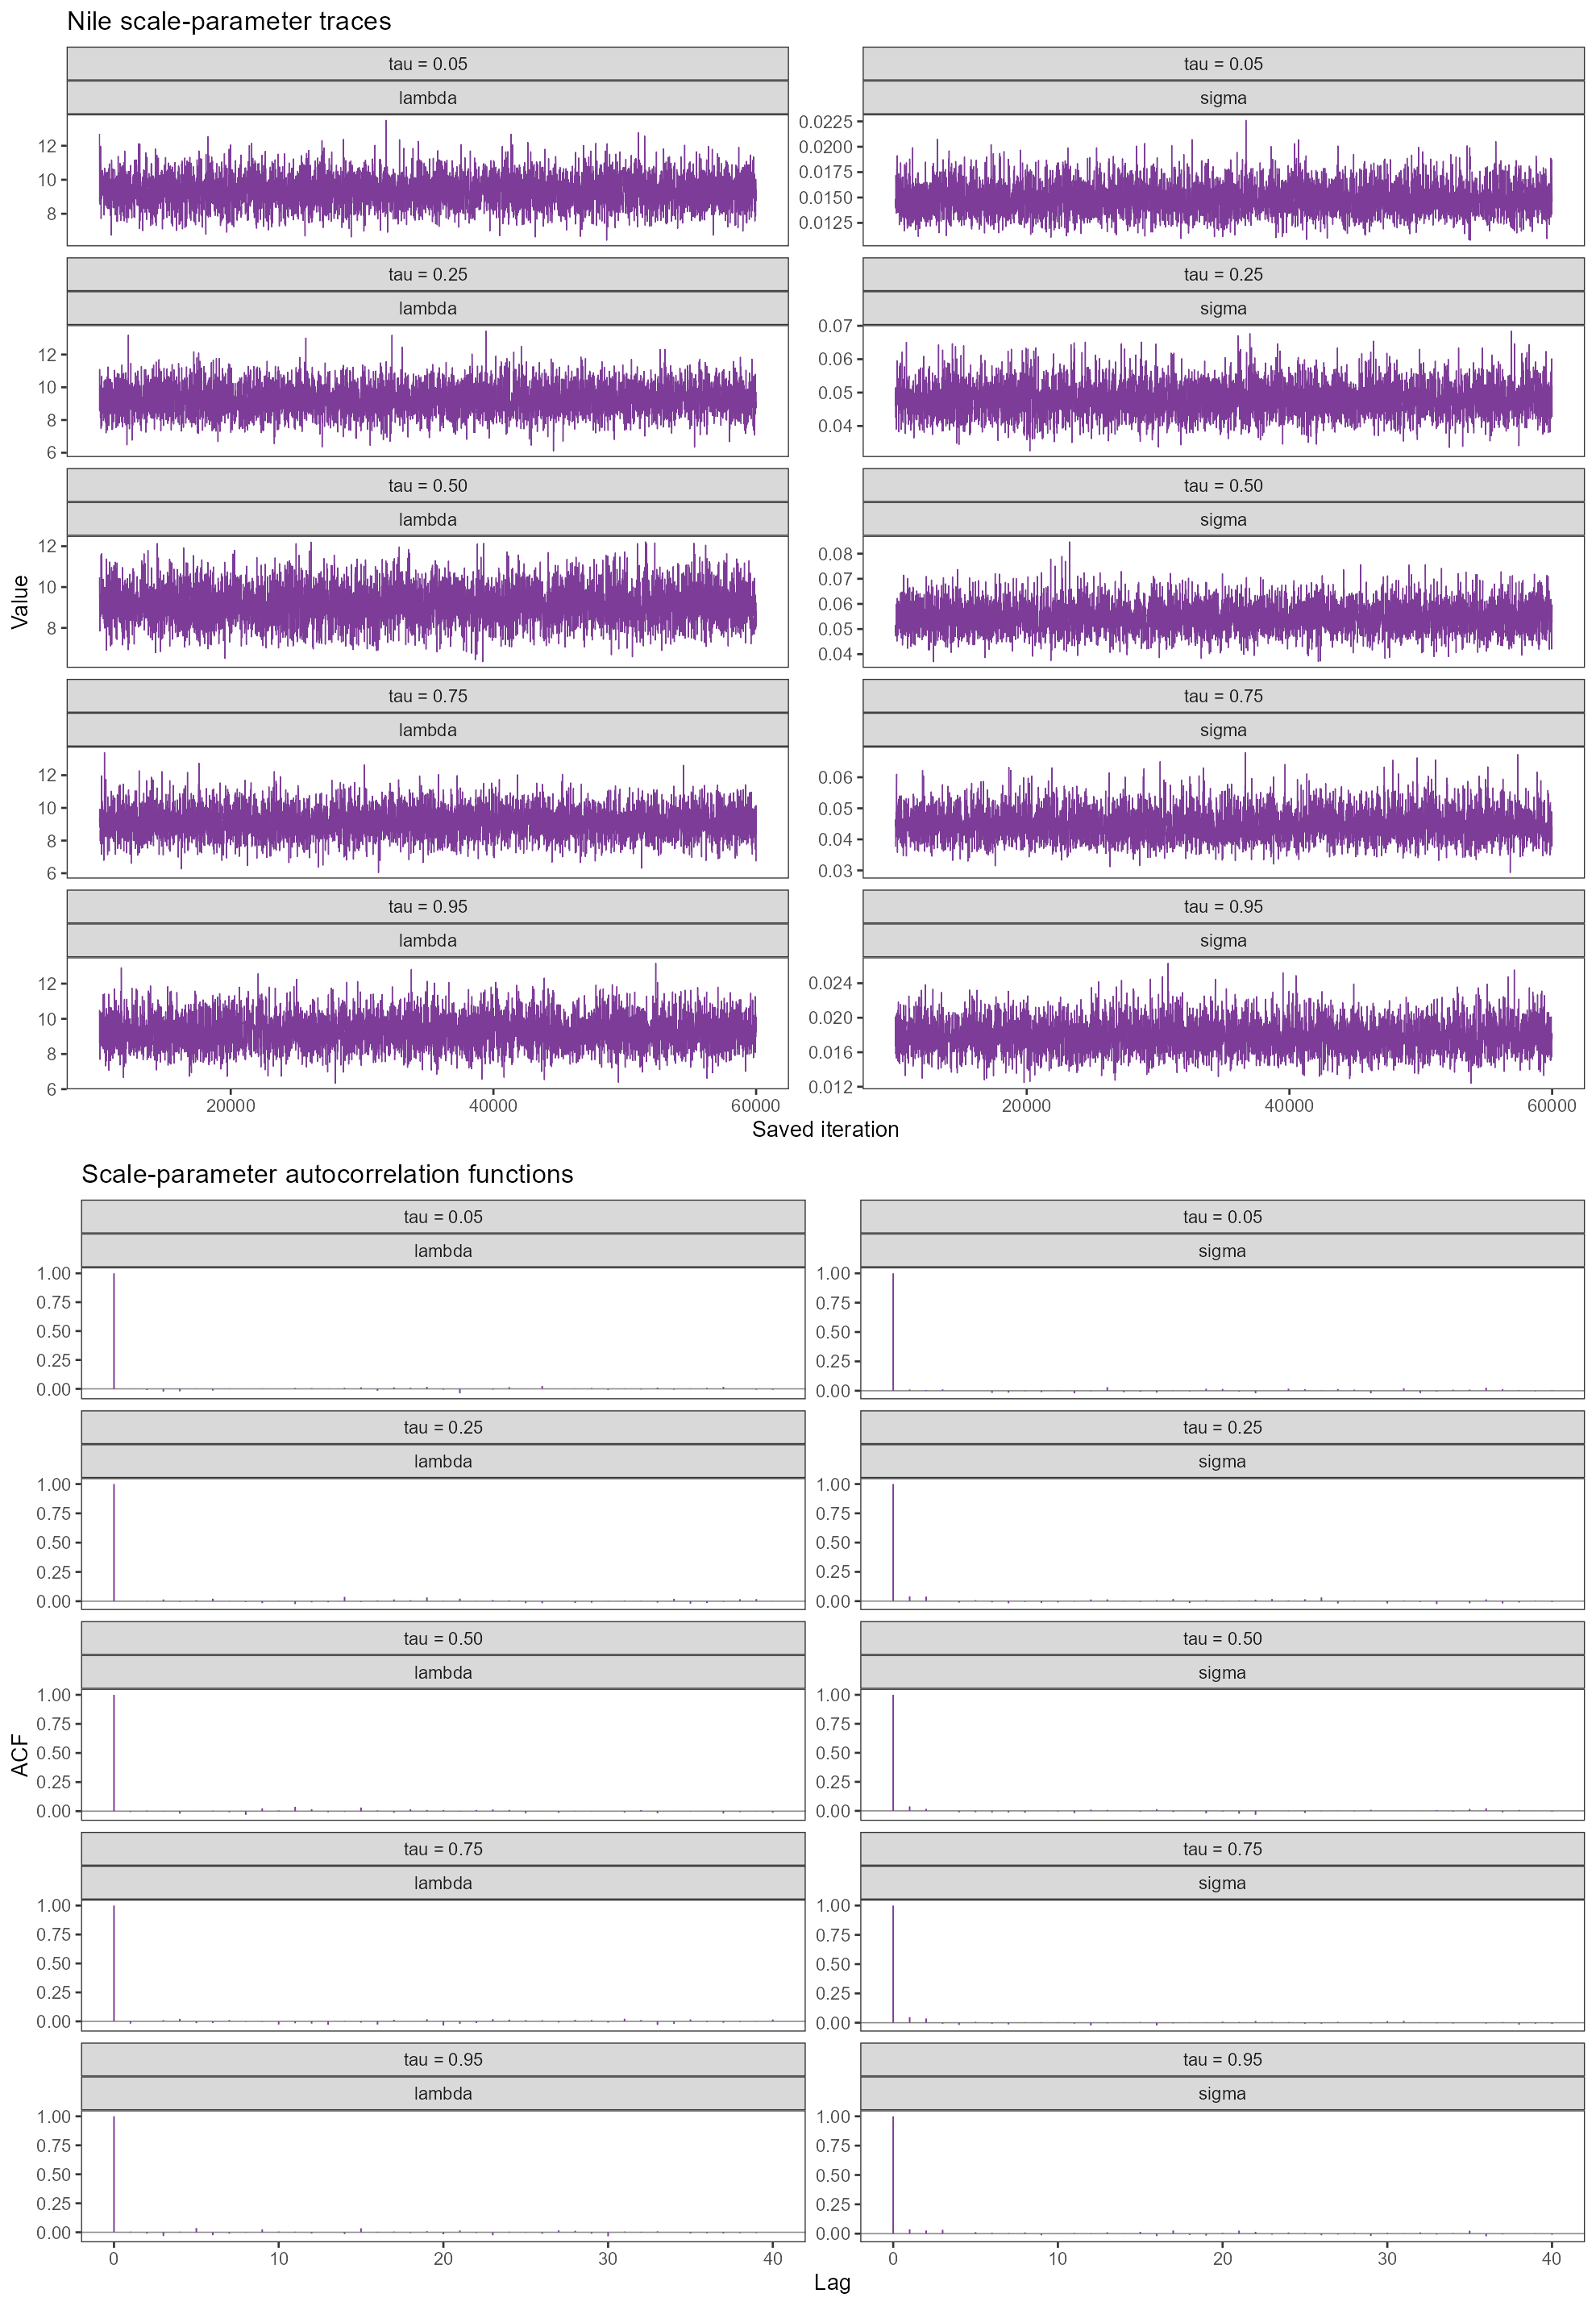
\includegraphics[width=0.75\textwidth,height=0.88\textheight,keepaspectratio]{figures/nile_scale_trace_acf_diagnostics}
	\caption{Nile trace and autocorrelation diagnostics for \(\lambda\) and \(\sigma\). Both scale-parameter chains mix rapidly and show no visible drift.}
	\label{fig:nile_scale_trace_acf}
\end{figure}

\begin{figure}[p]
	\centering
	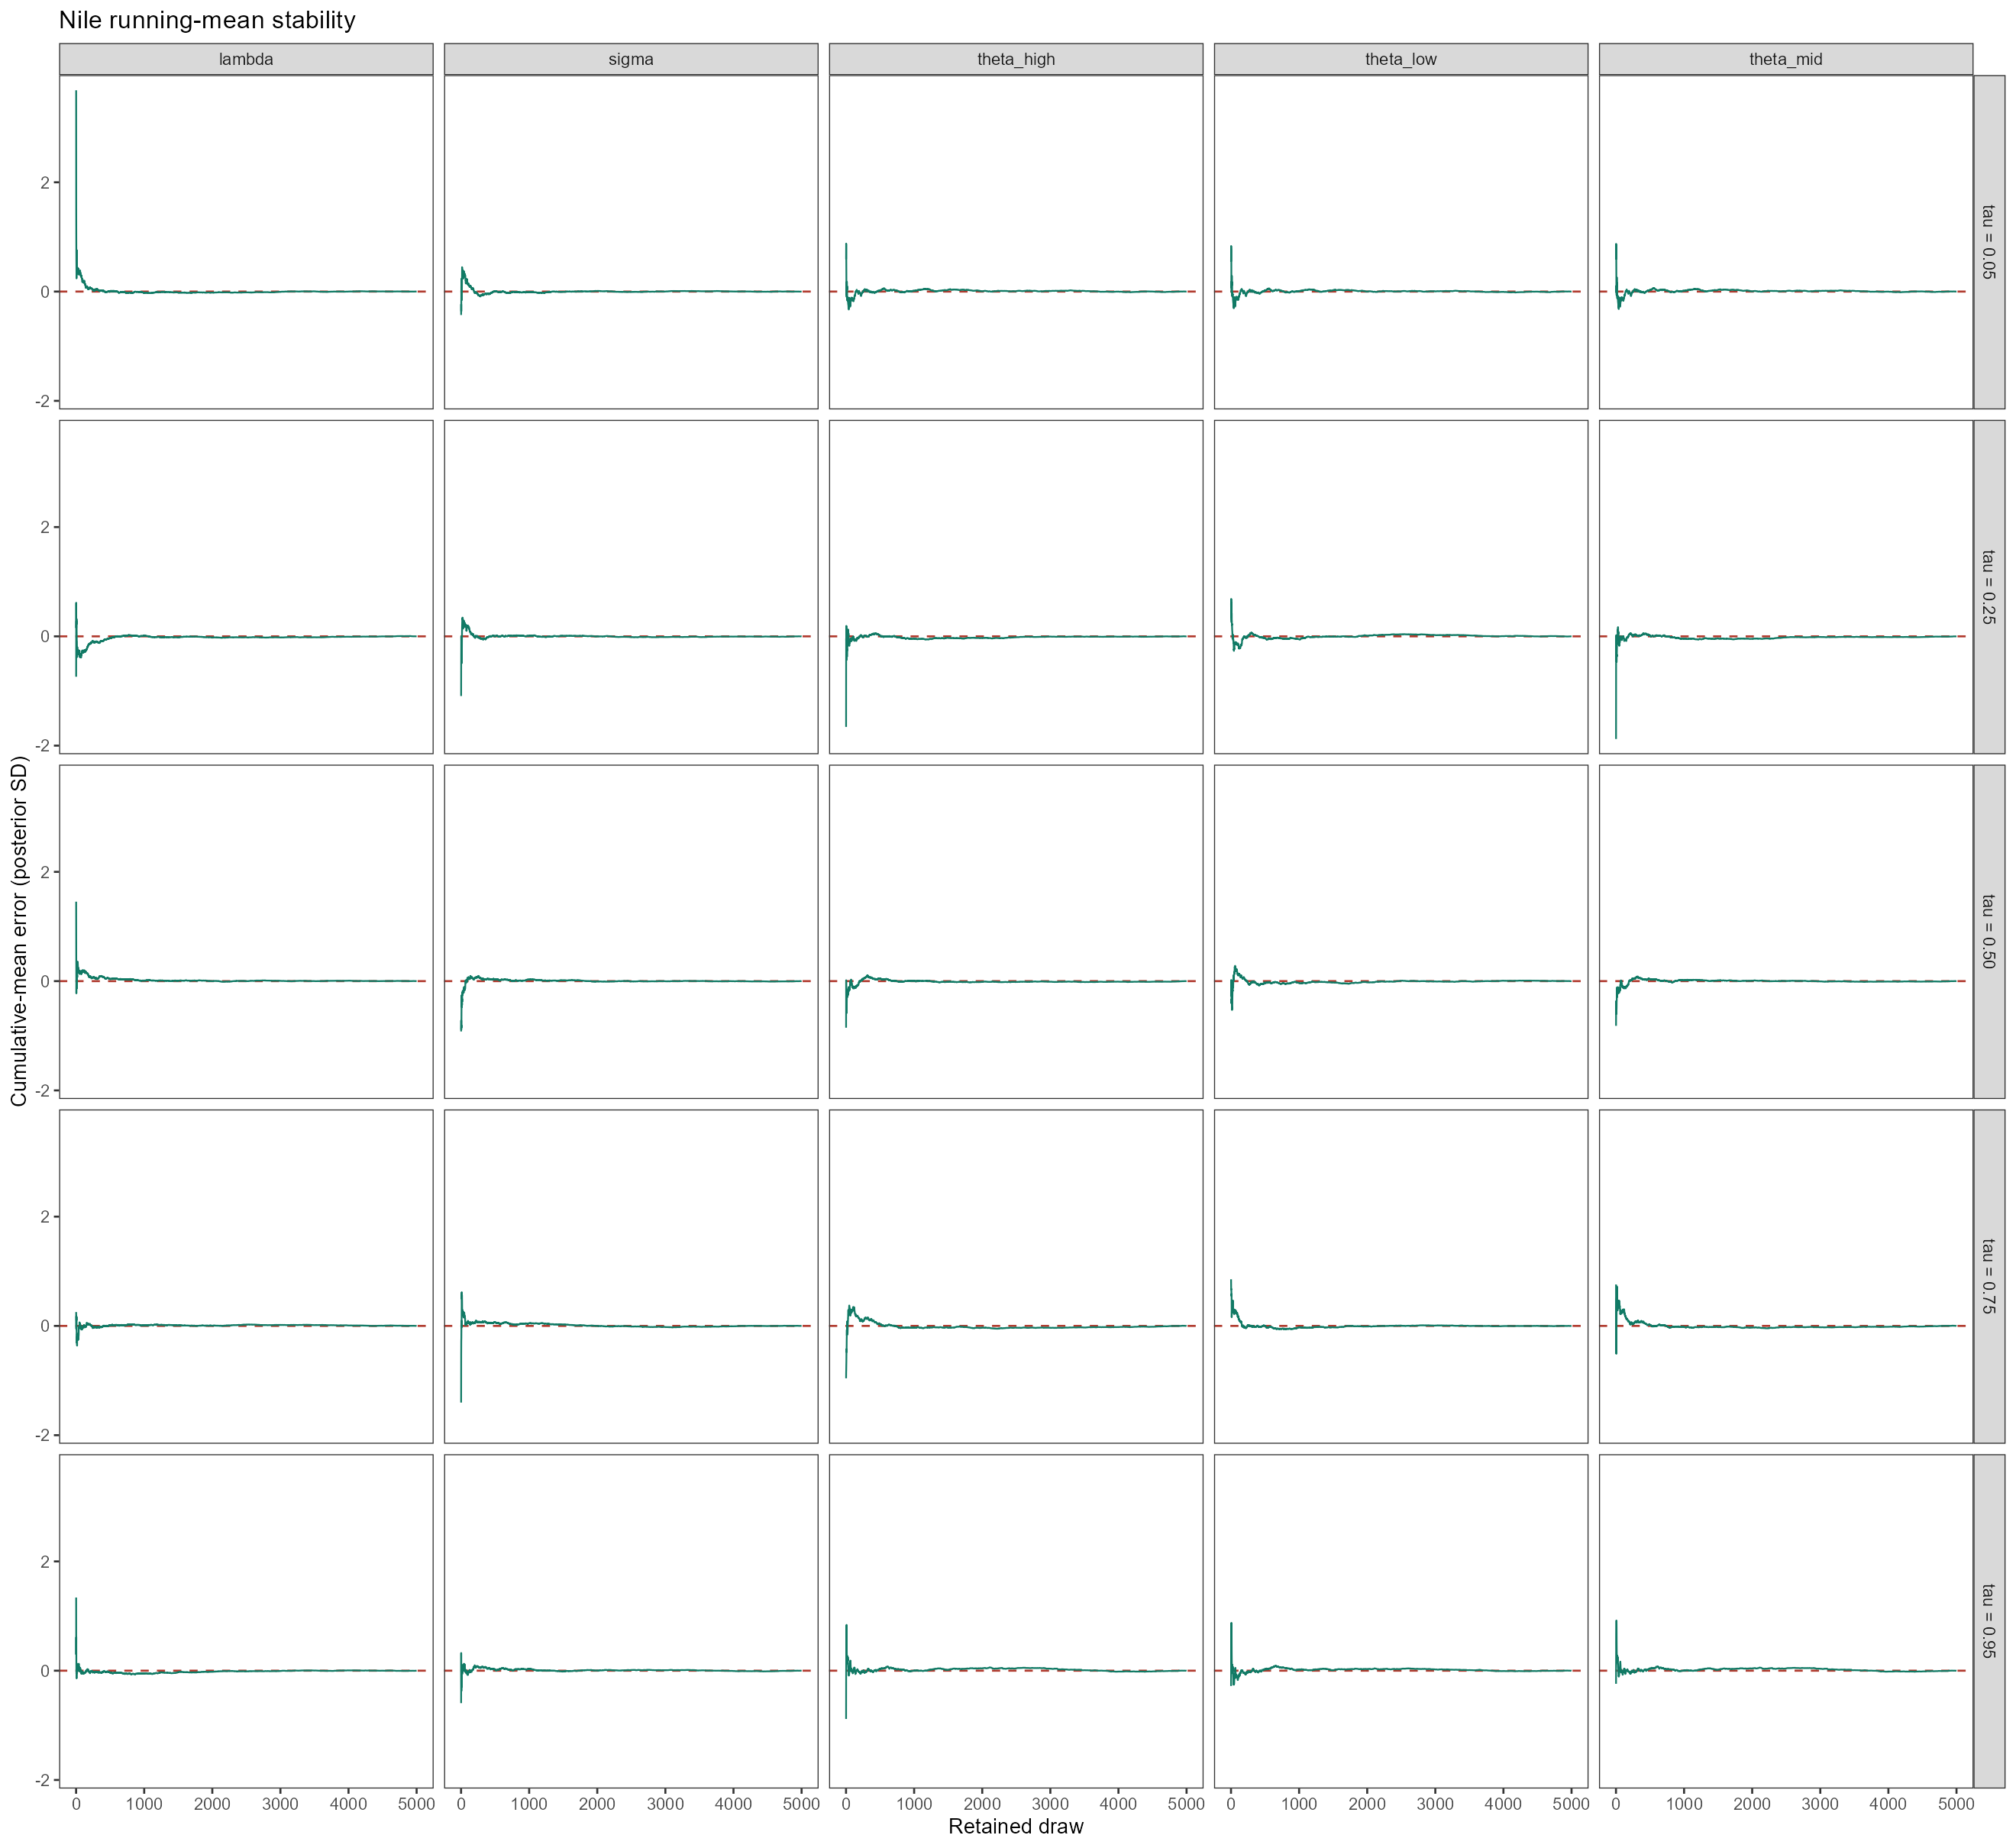
\includegraphics[width=0.75\textwidth,height=0.88\textheight,keepaspectratio]{figures/nile_running_mean_stability}
	\caption{Nile standardized cumulative-mean diagnostics. Each curve is the cumulative mean minus its final posterior mean, divided by the posterior standard deviation; the dashed line is zero.}
	\label{fig:nile_running_mean}
\end{figure}

\fi

\subsection{Growth Centiles}
\label{app:growth}

This appendix reports the growth-chart fits of Section~\ref{sec:app:growth} that are not shown there: the individual sampler for girls and the LMS centiles \citep{cole1992smoothing} for boys and girls. The P-MALA settings are those of Section~\ref{sec:app:growth}: $k = 2$, $\lambda \sim \mathrm{Gamma}(1,\sqrt{G})$, 6{,}000 iterations with 1{,}000 burn-in, and one independent run per level. The LMS curves are the 10th, 30th, 50th, 70th, and 90th centiles of the fitted Box--Cox Cole--Green distribution, evaluated on the same 0.1-year age grid.

\begin{figure}[htbp]
	\centering
	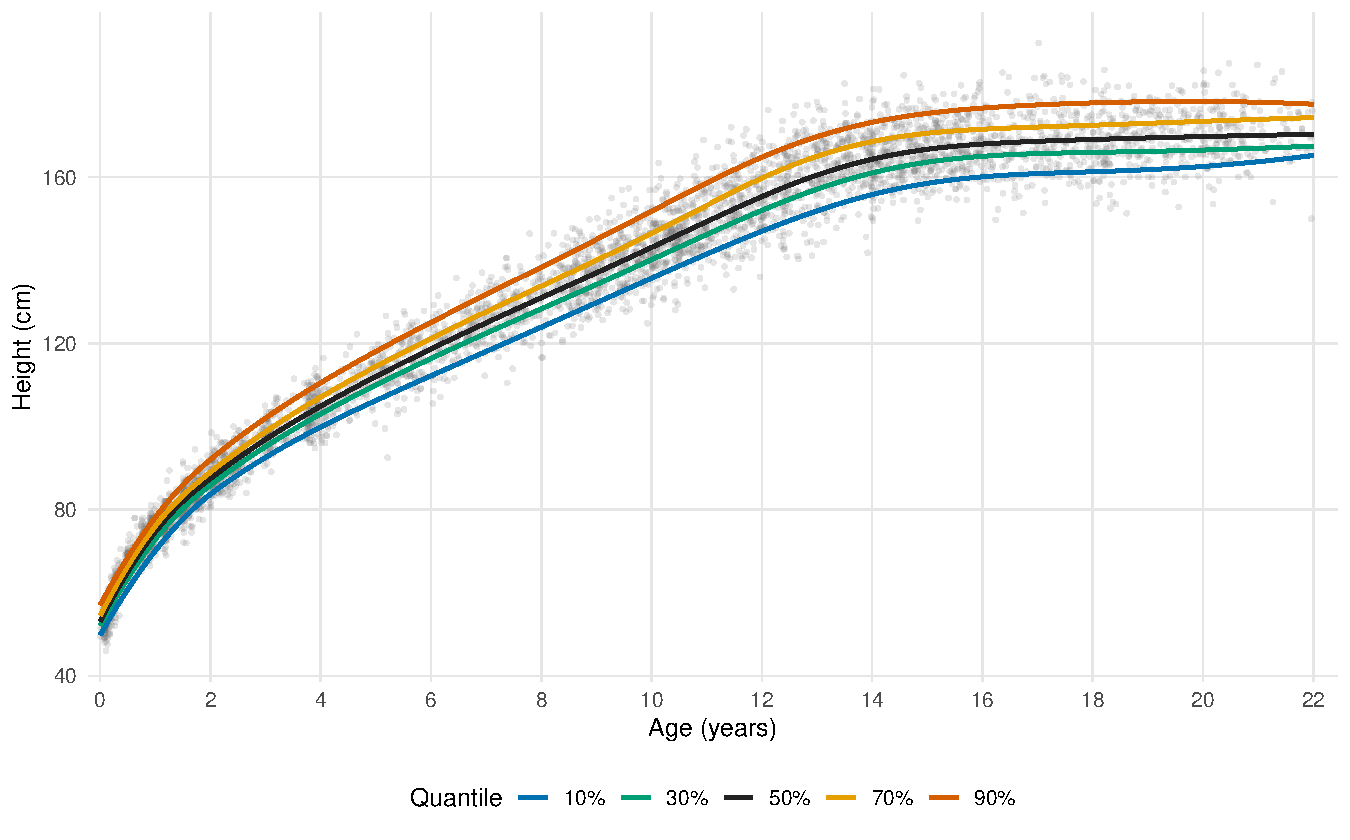
\includegraphics[width=0.75\textwidth]{figures/growth_pmala_girls}
	\caption{Individual P-MALA/Gibbs fits for the height of 5{,}190 Dutch girls (Fifth Dutch Growth Study, 2009) at $\tau \in \{0.1, 0.3, 0.5, 0.7, 0.9\}$, $k = 2$. Curves are posterior means on the 0.1-year age grid; grey circles are the individual measurements. Each level is fitted independently.}
	\label{fig:growth_girls}
\end{figure}

\begin{figure}[htbp]
	\centering
	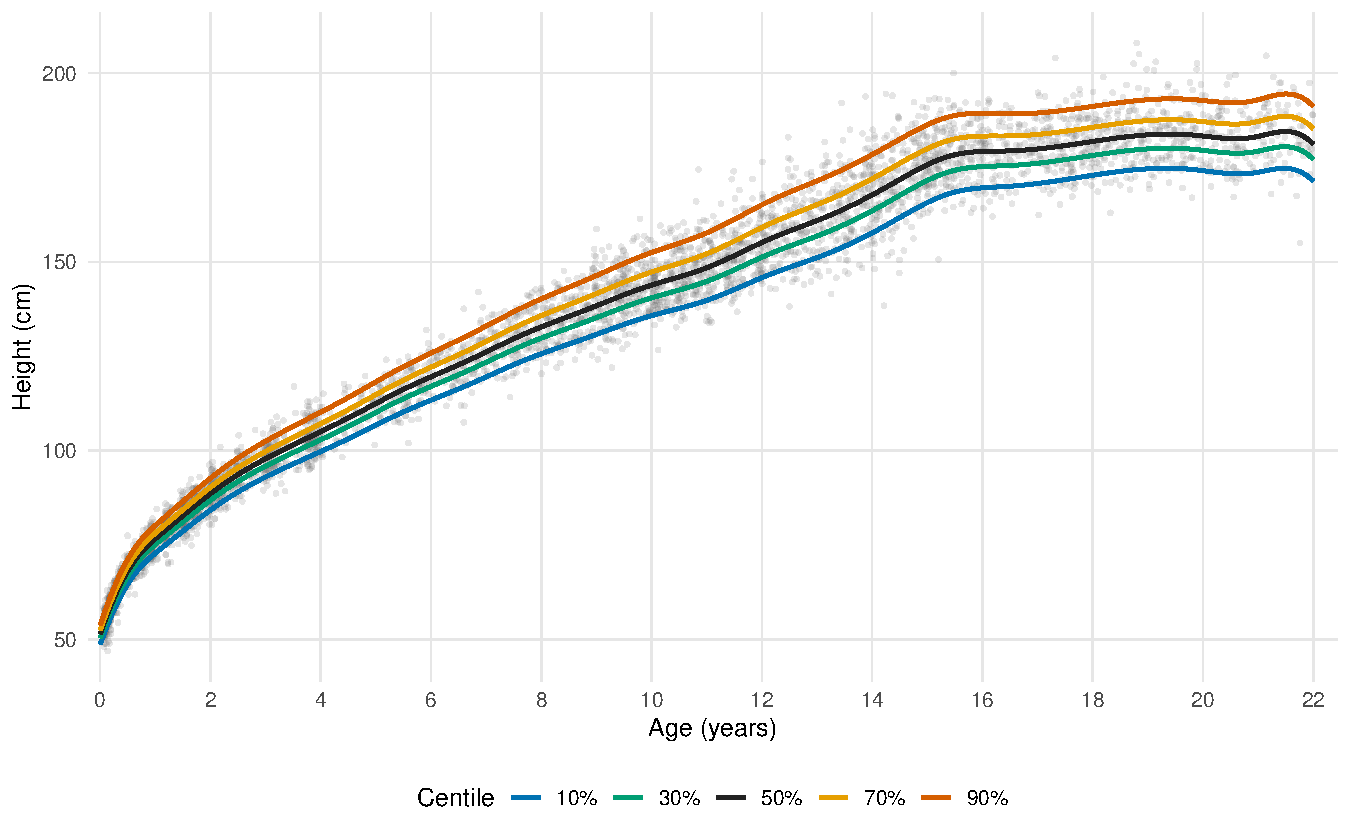
\includegraphics[width=0.75\textwidth]{figures/growth_lms_boys}
	\caption{LMS centiles for the height of 4{,}817 Dutch boys (Fifth Dutch Growth Study, 2009): the 10th, 30th, 50th, 70th, and 90th centiles of the fitted Box--Cox Cole--Green distribution, whose median, coefficient of variation, and Box--Cox power are smooth in age.}
	\label{fig:growth_lms_boys}
\end{figure}

\begin{figure}[htbp]
	\centering
	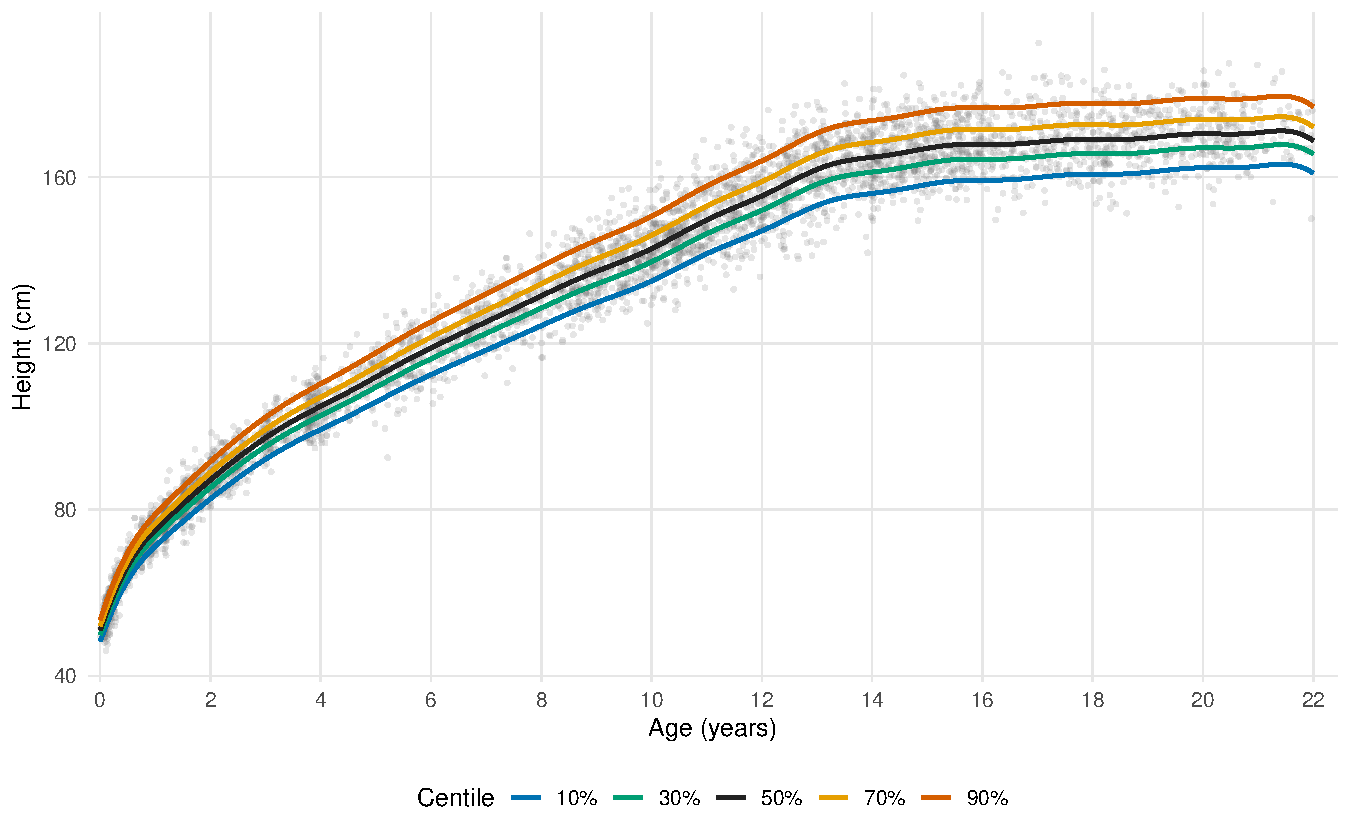
\includegraphics[width=0.75\textwidth]{figures/growth_lms_girls}
	\caption{LMS centiles for the height of 5{,}190 Dutch girls (Fifth Dutch Growth Study, 2009), with the layout of Figure~\ref{fig:growth_lms_boys}.}
	\label{fig:growth_lms_girls}
\end{figure}
